%%%%%%%%%%%%%%%%%%%%%%%%%%%%%%%%%%%%%%%%%%%%%%%%
%% Compile: PDFLaTeX BibTeX PDFLaTeX PDFLaTeX
%% Antonio Machicao y Priemer
%% Course: Wissenschaftliches Arbeiten (Homework)
%%%%%%%%%%%%%%%%%%%%%%%%%%%%%%%%%%%%%%%%%%%%%%%%

\documentclass[10pt,paper=a4,abstracton]{scrartcl}


%%%%%%%%%%%%%PACKAGES%%%%%%%%%%%%%

\usepackage[utf8]{inputenc}
\usepackage[english,ngerman]{babel}

\usepackage[T3,T1]{fontenc}
\usepackage{lmodern}
\usepackage{blindtext}

\usepackage{amsmath}
\usepackage{amssymb}
\usepackage{MnSymbol}

\usepackage[authoryear]{natbib}
	\setcitestyle{notesep={:~}}

\usepackage{graphicx}
%\usepackage{booktabs, array}

\usepackage[noenc,safe]{tipa}

%\usepackage{etex}		%For Forest bug
\usepackage[linguistics]{forest}
%\usepackage{tikz-qtree}

\usepackage{venndiagram}
\usepackage{vowel}

%\usepackage{xspace}
%\usepackage{setspace}
%\usepackage{listings}
%\usepackage{multicol}

%\usepackage[bookmarksnumbered]{hyperref}
\usepackage[bookmarksnumbered, 
	hidelinks
	]{hyperref}

%\usepackage{linguex}
%\usepackage{gb4e}
\usepackage{lsp-gb4eMyP}


%%%%%%%%%%%%%META DATA%%%%%%%%%%%%%
\author{$\langle$Ihr Name$\rangle$ \and $\langle$noch ein Name$\rangle$}

\title{\LaTeX\ für Linguisten}

\subtitle{Meine erste \LaTeX -Datei}

\date{$\langle$Das heutige Datum$\rangle$}


%%%%%%%%BEGIN DOCUMENT%%%%%%%%%%%%%
\begin{document}

\maketitle

\begin{abstract}
	Ein Abstract ist eine kurze Zusammenfassung über den Inhalt 
	der Arbeit. Das Abstract wird immer am Anfang des Dokuments 
	positioniert.\par
	Es ist auch möglich das Abstract in mehrere Absätze
	zu teilen.
\end{abstract}

\tableofcontents

\listoffigures

\listoftables


%%%%%%%%%%%%%%%%%%%%%%%%
\section{Hausaufgabe 1}


%%%%%%%%%%%%%%%%%%%%%%%%
\subsection[Zeichen und Sonderzeichen]{Hier werden Zeichen und Sonderzeichen geübt}

Folgende Zeichen können bei \LaTeX\ nicht direkt benutzt werden: \# \$ \& \_ \{ \} \%. Für die folgenden Zeichen braucht man andere Befehle: \textbackslash, \textgreater , \textless , \textasciicircum .


%%%%%%%%%%%%%%%%%%%%%%%%
\subsubsection[Erste Subsection]{Das ist eine Subsection}

Diese Datei ist dazu gemacht, dass alle Workshopteilnehmer einige Vorzüge von \LaTeX\ austesten können.


%%%%%%%%%%%%%%%%%%%%%%%%
\subsubsection[Zweite Subsection]{Das ist eine weitere Subsection}

Diese Datei ist dazu gemacht, dass alle Workshopteilnehmer einige Vorzüge von \LaTeX\ austesten können.


%%%%%%%%%%%%%%%%%%%%%%%%
\subsection[Fußnoten]{Hier werden Fußnoten geübt}

Diese Datei ist dazu gemacht, dass alle Workshopteilnehmer\footnote{Hier ist eine Fußnote.} einige Vorzüge von \LaTeX\ austesten können.\footnote{Hier ist noch eine Fußnote.}


%%%%%%%%%%%%%%%%%%%%%%%%
\subsection[Textauszeichnung]{Hier wird die Textauszeichnung geübt}

Diese Datei ist {\tiny dazu} gemacht, dass {\Huge alle} Workshopteilnehmer einige {\Large Vorzüge} von \LaTeX\ austesten können.

Diese \textbf{Datei} ist dazu \underline{gemacht}, dass alle \textsc{Workshopteilnehmer} einige \emph{Vorzüge} von \LaTeX\ austesten \texttt{können}.

\noindent Diese Datei ist dazu gemacht, dass alle Workshopteilnehmer einige Vorzüge von \LaTeX\ austesten können.


%%%%%%%%%%%%%%%%%%%%%%%%
\section{Hausaufgabe 2}


%%%%%%%%%%%%%%%%%%%%%%%%
\subsection{Textumgebungen}


%%%%%%%%%%%%%%%%%%%%%%%%
\subsubsection{Quote und Quotation}

 Diese Datei ist dazu gemacht, dass alle Workshopteilnehmer einige Vorzüge von \LaTeX\ austesten können. Das ist der Text vor der \texttt{quote}-Umgebung.
\begin{quote}
	Die grammatischen Phänomene in einer Sprache zerfallen in zwei Teilbereiche: kerngrammatische und randgrammatische Phänomene (\emph{Ausnahmen}).
	
	Die grammatischen Phänomene in einer Sprache zerfallen in zwei Teilbereiche: kerngrammatische und randgrammatische Phänomene (\emph{Ausnahmen}).
\end{quote}
Das ist der Text nach der \texttt{quote}-Umgebung. Diese Datei ist dazu gemacht, dass alle Workshopteilnehmer einige Vorzüge von \LaTeX\ austesten können.


 Diese Datei ist dazu gemacht, dass alle Workshopteilnehmer einige Vorzüge von \LaTeX\ austesten können. Das ist der Text vor der \texttt{quotation}-Umgebung.
\begin{quotation}
	Die grammatischen Phänomene in einer Sprache zerfallen in zwei Teilbereiche: kerngrammatische und randgrammatische Phänomene (\emph{Ausnahmen}).
	
	Die grammatischen Phänomene in einer Sprache zerfallen in zwei Teilbereiche: kerngrammatische und randgrammatische Phänomene (\emph{Ausnahmen}).
\end{quotation}
Das ist der Text nach der \texttt{quotation}-Umgebung. Diese Datei ist dazu gemacht, dass alle Workshopteilnehmer einige Vorzüge von \LaTeX\ austesten können.


%%%%%%%%%%%%%%%%%%%%%%%%
\subsubsection{Listen}

Diese Datei ist dazu gemacht, dass alle Workshopteilnehmer einige Vorzüge von \LaTeX\ austesten können.
 
\begin{itemize}
	\item Diese 
	\item Datei 
	\item[+] ist 
	\item dazu 
	\item gemacht
\end{itemize} 

Diese Datei ist dazu gemacht, dass alle Workshopteilnehmer einige Vorzüge von \LaTeX\ austesten können.

\begin{enumerate}
	\item Diese 
	\item Datei 
	\begin{enumerate}
		\item[+] ist 
		\item dazu 
		\item gemacht
	\end{enumerate}
	\item einige 
	\item Vorzüge 
	\item von 
	\item \LaTeX\ 
	\item auszutesten
\end{enumerate}

Diese Datei ist dazu gemacht, dass alle Workshopteilnehmer einige Vorzüge von \LaTeX\ austesten können.

\begin{description}
	\item[Linguistik:] eine wissenschaftliche Disziplin
	\begin{itemize}
		\item Ihr Untersuchungsobjekt ist die Sprache.
		\item Sie interagiert mit anderen Disziplinen:
		\begin{enumerate}
			\item Philosophie
			\item Psychologie
			\item Soziologie
		\end{enumerate}
	\end{itemize}
\end{description}


%%%%%%%%%%%%%%%%%%%%%%%%
\subsection{Nicht-textbezogene Umgebungen}


%%%%%%%%%%%%%%%%%%%%%%%%
\subsubsection{Paket installieren}

Das Paket \textbf{blindtext} wurde in der Präambel installiert und im Folgenden benutzt:


\blindtext



%%%%%%%%%%%%%%%%%%%%%%%%
\subsubsection{Grafiken}

Die folgende Grafik ist so breit wie der Text:

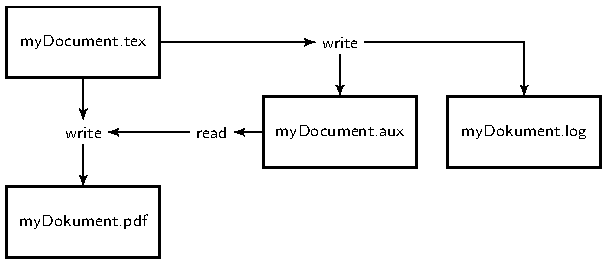
\includegraphics[width=\linewidth]{LaTeX_flowchart_1.pdf}


Die Größe der folgenden Grafik ist 50\% der Textbreite:

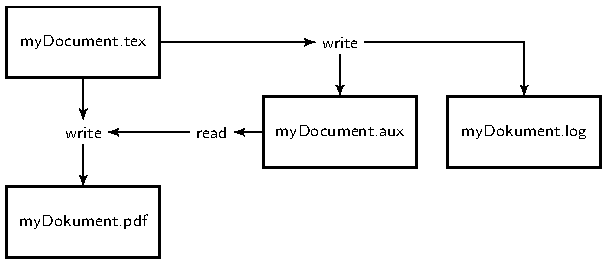
\includegraphics[width=.5\linewidth]{LaTeX_flowchart_1}


%%%%%%%%%%%%%%%%%%%%%%%%
\subsubsection{Tabellen}

Ein Beispiel einer Tabelle: 
\begin{tabular}[t]{rc|l|}
	ZelleZelle 1 & ZelleZelle 2 & ZelleZelle 3 \\
	ZelleZelle 1 & ZelleZelle 2 & ZelleZelle 3 \\
	\hline
	Zelle & Zelle & Zelle \\
\end{tabular}


%%%%%%%%%%%%%%%%%%%%%%%%
\subsubsection{Gleitumgebungen}

Die Größe der folgenden Grafik ist 50\% der Textbreite:

\begin{figure}[htbp]
	\centering
	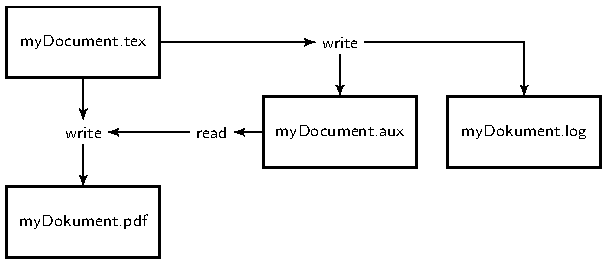
\includegraphics[width=.5\linewidth]{LaTeX_flowchart_1}
	\caption{Flowchart}
	\label{fig:flowchart}
\end{figure}


\blindtext


Ein Beispiel einer Tabelle in einer Gleitumgebung: 

\begin{table}[htbp]
\centering	
\caption{Meine erste Tabelle}
\begin{tabular}[t]{rc|l|}
	ZelleZelle 1 & ZelleZelle 2 & ZelleZelle 3 \\
	ZelleZelle 1 & ZelleZelle 2 & ZelleZelle 3 \\
	\hline
	Zelle & Zelle & Zelle \\
\end{tabular}
\label{fig:Tabelle1}
\end{table}


%%%%%%%%%%%%%%%%%%%%%%%%
\subsubsection{Querverweise}

Hier wird auf die Tabelle \ref{fig:Tabelle1} und hier auf die Abbildung \ref{fig:flowchart} referiert, die Abbildung befindet sich auf Seite \pageref{fig:flowchart}


%%%%%%%%%%%%%%%%%%%%%%%%
\section{Hausaufgabe 3}


%%%%%%%%%%%%%%%%%%%%%%%%
\subsection{Referenzen im Text}

\citeauthor{Chomsky80a} verfasste \citeyear{Chomsky80a} seinen Artikel \emph{On Binding}. \citeauthor{Chomsky80a}s Artikel wird sehr häufig zitiert \citep[vgl.][]{Heim&Kratzer00a}.


%%%%%%%%%%%%%%%%%%%%%%%%
\subsection{Verschiedene natbib-Befehle}

Im Folgenden sind verschiedene Beispiele für \texttt{natbib}-Befehle aufgelistet:

\begin{enumerate}
	\item \textbackslash citealt\{xxx\}: \citealt{Heim&Kratzer00a}
	
	\item \textbackslash citealp\{xxx\}: \citealp{Heim01a}
	
	\item \textbackslash citet\{xxx\}: \citet{Winter97a}  
	
	\item \textbackslash citet[aa]\{xxx\}: \citet[36]{Champollion14a}
	
	\item \textbackslash citep\{xxx\}: \citep{Krifka89a}
	
	\item \textbackslash citep[aa]\{xxx\}: \citep[42]{MyP17c} 
	
	\item \textbackslash citep[bb][aa]\{xxx\}: \citep[vgl.][36]{Nolda&Co14a}
	
	\item \textbackslash citep[bb][~]\{xxx\}: \citep[vgl.][]{Heusinger&Co11a} 
	
	\item \textbackslash citep[bb][~]\{xxx, yyy, zzz\}: \citep[vgl.][]{Heim01a,Winter97a,Krifka89a}
\end{enumerate}


%%%%%%%%%%%%%%%%%%%%%%%%
\section{Hausaufgabe 4}


%%%%%%%%%%%%%%%%%%%%%%%%
\subsection{Beispiele mit \texttt{lsp-gb4eMyP}}

Unter diesem Absatz stehen mehrere Beispielsätze, die mit dem Paket \texttt{gb4e} generiert wurden. Beispiel (\ref{ex:01}) besteht aus einer Ebene, während in (\ref{ex:02a}), sowie (\ref{ex:02b}) zwei Ebenen verwendet werden. 

\begin{exe}
	\ex \label{ex:01}
	Das ist ein Beispielsatz
	
	\ex 
	\begin{xlist} 
	\ex \label{ex:02a} Manchen Linguisten fällt es schwer, sich Beispielsätze zu überlegen.
	\ex \label{ex:02b} Dass viele Linguisten unkreativ sind, überrascht nicht.
	\end{xlist}
\end{exe}

Die Sätze in (\ref{ex:03}) zeigen Urteile über die Grammatikalität. Das Beispiel (\ref{ex:03b}) ist wohlgeformt und die Zeile ist aligniert. In (\ref{ex:04}) werden die Beispielsätze glossiert und übersetzt. 


\begin{exe}
	\ex \label{ex:03}
	
	\begin{xlist}
	\ex[*]{Manche Linguisten sich keine Gedanken über die Wortstellung machen.}
	
	\ex[]{dass sich manche Linguisten keine Gedanken über die Worstellung machen}\label{ex:03b}
	
	\ex[?]{Andere Beispiele sind markiert nur.}
	\end{xlist}

	\ex 
	\begin{xlist}
			
	\ex \label{ex:04}
	\gll Dass viele Linguist-inn-en Grammatik mögen, überrascht nicht. \\
	that many linguist-\textsc{fem}-\textsc{pl} grammar like.\textsc{3pl} surprises not\\
	\glt \glq{}That many linguists like grammar is not surprising.\grq{}

	\ex 
	\gll Auch Mehrwortelemente können glossiert werden.\\
	also {more.word.elements} can.\textsc{3pl} glossed be\\

	\end{xlist}

\end{exe}


%%%%%%%%%%%%%%%%%%%%%%%%
\subsection{Beispiele mit \texttt{lsp-gb4eMyP} und \texttt{tipa}}

Mit dem Paket \texttt{tipa} können IPA-Symbole dargestellt werden.

\eal\label{ex:05}
\ex \textipa{[PUm.StK\texttoptiebar{OI}.n@n]}
\ex \textipa{[\textsecstress Ekspl@"neIS@n]}
\zl 


%%%%%%%%%%%%%%%%%%%%%%%%
\subsection{Strukturbäume mit \texttt{forest}}

Der Baum in (\ref{ex:06}) wurde mit dem Paket \texttt{forest} erstellt und ist zusätzlich in eine Beispielumgebung eingebettet.

\begin{exe}

\ex \label{ex:06}
\begin{forest}
	[CP, draw, red
	[DP$_{1}$, name=T12 [Syntaktiker, roof]]
	[C$^{\prime}$
		[C$^{0}$ [zeichnen$_{2}$]]
			[TP, fill=blue [$t_{1}$, name=T11]
			[T$^{\prime}$
				[VP, fill=red [$t_{1}$, name=T10]
				[V$^{\prime}$ [DP [Bäume,roof]]
				[V$^{0}$ [$t_{2}$]]]]
			[T$^{0}$ [$t_{2}$]]
			]]]
	]
	\draw[->] (T10) to[out=south west, in=south west](T11);
	\draw[->] (T11) to[out=south west, in=south west](T12);
\end{forest}
\end{exe}


\clearpage


%%%%%%%%%%%%%%%%%%%%%%%
\subsection{Venndiagramme mit \texttt{venndiagram}}
\begin{figure}[h!]
\centering
\begin{venndiagram3sets}[
	labelOnlyA={1},
	labelOnlyB={2},
	labelOnlyC={3},
	labelOnlyAB={4},
	labelOnlyAC={5},
	labelOnlyBC={6},
	labelABC={7},
	labelNotABC={8}
	]
	\fillACapBCapC
\end{venndiagram3sets}
\begin{venndiagram3sets}[
	labelOnlyA={1},
	labelOnlyB={2},
	labelOnlyC={3},
	labelOnlyAB={4},
	labelOnlyAC={5},
	labelOnlyBC={6},
	labelABC={7},
	labelNotABC={8}
	]
	\fillNotABC
\end{venndiagram3sets}
\caption{Zwei Venndiagramme}
\end{figure}


%%%%%%%%%%%%%%%%%%%%%%%%
\subsection{Vokalviereck mit \texttt{vowel}}
~
\begin{figure}[h!]
\centering
{\LARGE
\begin{vowel}
	\putcvowel[l]{\textipa{i:}}{1}
	\putcvowel[r]{\textipa{y:}}{1}
	\putcvowel[l]{\textipa{e:}}{2}
	\putcvowel[r]{\textipa{\o:}}{2}
	\putcvowel[l]{\textipa{\textepsilon~\textepsilon:}}{3}
	\putcvowel[r]{\oe}{3}
	\putcvowel[r]{\textipa{\textopeno}}{6}
	\putcvowel[r]{\textipa{o:}}{7}
	\putcvowel[r]{\textipa{u:}}{8}
	\putcvowel{\textschwa}{11}
	\putcvowel{\textsci\ \textscy}{13}
%	\putvowel[l]{a}{3\vowelhunit}{3\vowelvunit}
	\putvowel[l]{\textipa{a}}{3\vowelhunit}{3\vowelvunit}
	\putvowel[r]{\textipa{a:}}{3\vowelhunit}{3\vowelvunit}
\end{vowel}
}
\caption{Die Vokale des Deutschen}
\end{figure}


\clearpage


%%%%%%%%%%%%%%%%%%%%%%%%
\section{Hausaufgabe 6}


%%%%%%%%%%%%%%%%%%%%%%%%
\subsection{Der Mathematikmodus}
Der Mathematikmodus kann entweder inline oder im Display-Stil verwendet werden:
Wenn $2^2+\sqrt{16}=4+c^2$, wie viel beträgt $c$? \\
Wenn \[2^2+\sqrt{16}=4+c^2\] wie viel beträgt $c$?

In \eqref{eq:FirstEq} wurde die \texttt{equation}-Umgebung genutzt um die Gleichung zu nummerieren. Mit dem Befehl \texttt{\textbackslash{}eqref\{xxx\}} kann auf die Gleichung verwiesen werden.

\begin{equation}
\label{eq:FirstEq}
2^2+\sqrt{16}=4+2^2
\end{equation}


%%%%%%%%%%%%%%%%%%%%%%%
\subsection{Mengenlehre}

\eal
\ex $\{\textrm{a}\} \subset \{\textrm{a, e}\}$
\ex $\emptyset \subseteq \{\textrm{a, b}\}$
\ex $\# \{\emptyset, \textrm{a} \} = 2$
\ex $\emptyset \in \{\emptyset, \textrm{a} \}$
\zl 


%%%%%%%%%%%%%%%%%%%%%%%
\subsection{Aussagenlogik}

\eal
\ex $(A \lor B ) \lor C \Leftrightarrow A \lor ( B \lor C)$
\ex $(A \land B ) \land C \Leftrightarrow A \land ( B \lor C)$
\zl

\eal
\ex $\lnot (A \Rightarrow B) \Leftrightarrow A \land \lnot B$ 
\ex $\lnot (A \Leftrightarrow B) \Leftrightarrow (A \Leftrightarrow \lnot B)$ 
\zl 


%%%%%%%%%%%%%%%%%%%%%%%
\subsection{Quantoren}

\eal
\ex $\exists x [$\textsc{studentin}$(x)$ $\land $ \textsc{lesen}$(x)]$
\ex $\forall x [$\textsc{studentin}$(x)$ $\rightarrow $ \textsc{lesen}$(x)]$
\zl 


%%%%%%%%%%%%%%%%%%%%%%%
\subsection{Klammern}
\eal
\ex $\lsem \alpha \beta \rsem = \lsem \beta \rsem (\lsem \alpha \rsem)$
\ex $\langle e, t \rangle$
\ex \emph{Achtung} enthält den Digraphen $\langle$ch$\rangle$
\zl 


%%%%%%%%%%%%%%%%%%%%%%%
%% LITERATUR

\bibliographystyle{deChicagoMyP}
%\bibliographystyle{chicago}
\bibliography{myLibrary}


\end{document}
%%%%%%%%END DOCUMENT%%%%%%%%%%%%%
